\documentclass[11pt]{article}

\usepackage[margin=1in]{geometry}
\usepackage{amsmath, amssymb, amsfonts, amsthm}
\usepackage{enumitem}
\usepackage[colorlinks=true, linkcolor=blue, urlcolor=blue]{hyperref}
\usepackage{tikz}
\usetikzlibrary{arrows.meta,calc,positioning,decorations.pathreplacing}

\theoremstyle{plain}
\newtheorem{theorem}{Theorem}[section]
\newtheorem{lemma}[theorem]{Lemma}
\newtheorem{proposition}[theorem]{Proposition}
\newtheorem{corollary}[theorem]{Corollary}
\theoremstyle{definition}
\newtheorem{definition}[theorem]{Definition}
\newtheorem{example}[theorem]{Example}
\theoremstyle{remark}
\newtheorem{remark}[theorem]{Remark}

\newcommand{\g}{\mathfrak{g}}
\newcommand{\R}{\mathbb{R}}
\newcommand{\Q}{\mathbb{Q}}
\newcommand{\pr}{\operatorname{pr}}
\newcommand{\Dx}{D_x}
\newcommand{\Dt}{D_t}

\title{\bf The Pure Mathematics Behind the LieML Engine:\\
jets, kernels, windows, and quotients}
\author{LieML project --- demonstration companion to \texttt{CURRICULUM.md}}
\date{2026-07-14}

\begin{document}
\maketitle

\begin{abstract}
\noindent This note demonstrates, by hand and with proofs, the mathematical claims that the LieML
curriculum rests on. Its standard of ``demonstration'' is concrete: \emph{every measured number that
the symmetry engine produced during validation is re-derived here in closed form} --- the Burgers
window sequence $[4,5,5]$, the heat sequence $[6,8,10,11,12]$, and the transport sequence
$[10,22,40,65,98]$, the last as an exact theorem
$\dim_D=2\binom{D+2}{2}+\binom{D+3}{3}$ whose proof takes six lines. Along the way we prove the four
structural facts that license the machine's design: the stage is forced (jet bundles), the group is a
kernel (linearity of the determining operator), the window is a filtration (monotone lower bounds),
and the parameter dependence is semicontinuous (jumps only up, only on thin sets). Two further
machine checks are then demonstrated with proofs and verified verdict tables for all five canonical
equations: the \emph{homogeneity check} --- an exact scaling-weight criterion decided by the
exponents alone, which emits scaling generators without ever building the determining matrix ---
and the \emph{solvability checks}: Kovalevskaya form before the kernel computation, the derived
series (Lie's quadrature theorem) after it. All symbolic claims are independently re-verified by
\texttt{symm/curriculum\_checks.py} (36/36 checks pass).
\end{abstract}

\tableofcontents

%======================================================================
\section{Introduction: what is being demonstrated}

The operating document \texttt{CURRICULUM.md} makes four load-bearing assertions:

\begin{enumerate}[nosep]
\item[(A)] the \emph{manifold} on which symmetry analysis happens is not selected by any algorithm
  --- it is forced by the PDE's signature (\S\ref{sec:stage});
\item[(B)] the \emph{group} is not guessed --- its Lie algebra is the kernel of a linear operator,
  and ``validity'' of a generator is an identity a machine can certify (\S\ref{sec:kernel});
\item[(C)] the engine's polynomial \emph{window} computes a certified, monotone lower bound
  $\dim_D$, whose exact behaviour on the three canonical test equations we can predict by hand
  (\S\ref{sec:window});
\item[(D)] symmetry dimension depends \emph{semicontinuously} on equation parameters --- constant
  generically, jumping only upward on thin special sets --- which forces the division of labor
  ``machine prioritizes, engine verifies'' (\S\ref{sec:param});
\item[(E)] two cheap structural checks bracket the kernel computation: the \emph{homogeneity}
  (scaling-weight) criterion, exact and decided by the term exponents alone, and the
  \emph{solvability} checks --- Kovalevskaya form before, the derived series after
  (\S\ref{sec:checks}).
\end{enumerate}

Section~\ref{sec:quotient} completes the story with the reduction step (algebra $\to$ quotient
manifold $\to$ ODE), and \S\ref{sec:license} states exactly which decision of the machine each
result licenses. Notation: independent variables $(x,t)$, dependent $u$; a point generator is
\[
X \;=\; \xi(x,t,u)\,\partial_x + \tau(x,t,u)\,\partial_t + \varphi(x,t,u)\,\partial_u .
\]

%======================================================================
\section{The stage is forced: jet space}\label{sec:stage}

\begin{definition}[Jet space]
For the scalar $(1{+}1)$ setting, the $k$-th \textbf{jet space} $J^k$ is the finite-dimensional
manifold with coordinates
\[
\big(x,\;t,\;u,\;u_x,\;u_t,\;u_{xx},\;u_{xt},\;u_{tt},\;\dots\big),
\qquad\text{all derivative symbols up to total order } k,
\]
where each derivative symbol is an \emph{independent coordinate}. The \textbf{total derivatives}
\[
\Dx=\partial_x+\sum_{a,b} u_{(a+1,b)}\,\frac{\partial}{\partial u_{(a,b)}},
\qquad
\Dt=\partial_t+\sum_{a,b} u_{(a,b+1)}\,\frac{\partial}{\partial u_{(a,b)}}
\]
are the vector fields that encode ``differentiate a formula as if the jet coordinates were honest
derivatives.'' A $k$-th order PDE $\Delta=0$ is a hypersurface
$\mathcal S_\Delta=\{\Delta=0\}\subset J^k$ (a submanifold wherever $d\Delta\neq0$), and a function
$u=f(x,t)$ solves the PDE iff its prolongation --- the graph
$(x,t,f,f_x,f_t,\dots)$ --- lies inside $\mathcal S_\Delta$.
\end{definition}

There is no choice anywhere in this construction: the number of independent variables, of dependent
variables, and the order $k$ read off the PDE determine $J^k$ completely. Figure~\ref{fig:stage}
shows the resulting geometry, including where the group will act and where the reduction will land.

\begin{figure}[ht]\centering
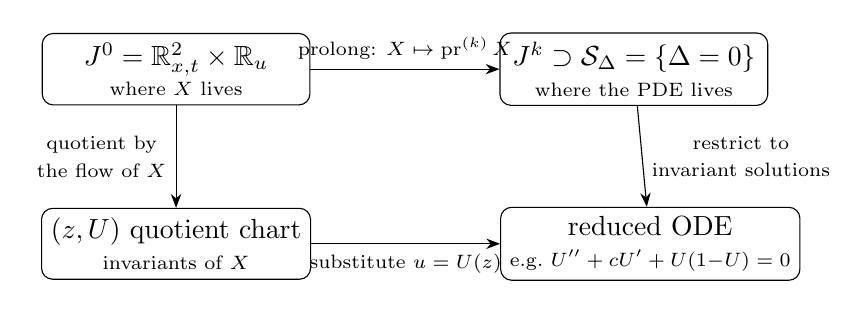
\begin{tikzpicture}[>={Stealth[length=5pt]}, node distance=9mm, every node/.style={align=center}]
  \node[draw, rounded corners, minimum width=34mm, minimum height=9mm] (J0)
    {$J^0=\R^2_{x,t}\times\R_u$\\[-1pt]{\scriptsize where $X$ lives}};
  \node[draw, rounded corners, minimum width=34mm, minimum height=9mm, right=24mm of J0] (Jk)
    {$J^k \supset \mathcal S_\Delta=\{\Delta=0\}$\\[-1pt]{\scriptsize where the PDE lives}};
  \node[draw, rounded corners, minimum width=34mm, minimum height=9mm, below=13mm of J0] (Q)
    {$(z,U)$ quotient chart\\[-1pt]{\scriptsize invariants of $X$}};
  \node[draw, rounded corners, minimum width=34mm, minimum height=9mm, right=24mm of Q] (ODE)
    {reduced ODE\\[-1pt]{\scriptsize e.g.\ $U''+cU'+U(1{-}U)=0$}};
  \draw[->] (J0) -- node[above]{\scriptsize prolong: $X\mapsto\pr^{(k)}X$} (Jk);
  \draw[->] (J0) -- node[left]{\scriptsize quotient by\\[-2pt]\scriptsize the flow of $X$} (Q);
  \draw[->] (Jk) -- node[right]{\scriptsize restrict to\\[-2pt]\scriptsize invariant solutions} (ODE);
  \draw[->] (Q) -- node[below]{\scriptsize substitute $u=U(z)$} (ODE);
\end{tikzpicture}
\caption{The four spaces of the subject. Top row: analysis (does $X$ preserve $\mathcal S_\Delta$?).
Bottom row: synthesis (use $X$'s invariants to collapse the PDE). Nothing on the top row is chosen;
everything on the bottom row is parametrized by the algebra computed on the top row.}
\label{fig:stage}
\end{figure}

%======================================================================
\section{The group is a kernel}\label{sec:kernel}

The generator acts on derivative coordinates through its \textbf{prolongation}
$\pr^{(k)}X = X + \sum_{1\le a+b\le k}\varphi^{(a,b)}\,\partial/\partial u_{(a,b)}$, with
coefficients defined recursively (exactly as implemented in \texttt{symm/sym\_engine/jet.py}):
\begin{equation}\label{eq:prolong}
\varphi^{(0,0)}=\varphi,\qquad
\varphi^{(a+1,b)}=\Dx\varphi^{(a,b)}-u_{(a+1,b)}\,\Dx\xi-u_{(a,b+1)}\,\Dx\tau,
\end{equation}
and symmetrically for the $t$-step. $X$ is a \textbf{point symmetry} of $\Delta=0$ iff
\begin{equation}\label{eq:inv}
\pr^{(k)}X(\Delta)\big|_{\Delta=0}=0 .
\end{equation}

\begin{lemma}[Linearity of the determining operator]\label{lem:linear}
For a fixed PDE $\Delta$, the map
\[
L:\;(\xi,\tau,\varphi)\;\longmapsto\;\pr^{(k)}X(\Delta)\big|_{\Delta=0}
\]
is $\R$-linear in $(\xi,\tau,\varphi)$ and their partial derivatives --- even when $\Delta$ is
nonlinear.
\end{lemma}

\begin{proof}
By induction on the recursion \eqref{eq:prolong}. The base coefficient $\varphi^{(0,0)}=\varphi$ is
linear. The inductive step applies $\Dx$ (a linear operator) to a quantity linear in the unknowns,
then subtracts jet coordinates ($u_{(a+1,b)}$, $u_{(a,b+1)}$ --- \emph{fixed} functions on $J^k$,
independent of the unknowns) times $\Dx\xi$, $\Dx\tau$, which are linear. Hence every
$\varphi^{(a,b)}$ is linear in the unknowns. Finally
$\pr^{(k)}X(\Delta)=\xi\,\partial_x\Delta+\tau\,\partial_t\Delta+\varphi\,\partial_u\Delta
+\sum\varphi^{(a,b)}\,\partial\Delta/\partial u_{(a,b)}$
is a sum of the unknowns and their prolongation coefficients multiplied by \emph{fixed} functions of
the jet coordinates; the on-shell restriction is a substitution of jet coordinates, which does not
touch the unknowns. Linearity is preserved throughout.
\end{proof}

\begin{theorem}[Classical; Olver]\label{thm:algebra}
The solution set $\g=\ker L$ is closed under the commutator $[X,Y]=XY-YX$, because prolongation is
a Lie-algebra morphism, $\pr[X,Y]=[\pr X,\pr Y]$. Hence the point symmetries of a PDE form a
\emph{Lie algebra}, not merely a vector space.
\end{theorem}

\begin{corollary}[What ``the machine points to a valid group'' actually means]\label{cor:valid}
Since $L$ is linear, expanding the residual $L(\xi,\tau,\varphi)$ in the free jet coordinates and
equating coefficients to zero yields a linear system --- the \textbf{determining matrix} $A$ over
$\Q$ --- whose null space \emph{is} the algebra. ``Valid'' is therefore not a judgment call:
$X$ is valid iff its residual \eqref{eq:inv} is the zero function, an identity checkable in exact
arithmetic. The engine certifies every generator this way, and the group is recovered from $\g$ by
exponentiating the flows.
\end{corollary}

This is assertion (B): nothing ``searches'' for the group. The group was always the kernel; all
genuine decisions live elsewhere --- in the window (\S\ref{sec:window}), the sweep order
(\S\ref{sec:param}), and the choice of subalgebra for reduction (\S\ref{sec:quotient}).

%======================================================================
\section{The window is a filtration: three sequences explained}\label{sec:window}

The engine searches $\g$ inside the finite-dimensional ansatz space
\[
V_D=\{\text{polynomials in }(x,t,u)\text{ of total degree}\le D\},\qquad
(\xi,\tau,\varphi)\in V_D^{\,3},
\]
and reports $\dim_D=\dim\big(\g\cap V_D^{\,3}\big)$, increasing $D$ until stabilization.

\begin{lemma}[Monotone certified lower bounds]\label{lem:window}
$\g\cap V_D^{\,3}\subseteq \g\cap V_{D+1}^{\,3}$, hence
$\dim_1\le\dim_2\le\cdots\le\dim\g$, and every $\dim_D$ is a \emph{certified lower bound} for
$\dim\g$: each of its $\dim_D$ basis vectors is a genuine symmetry (residual $\equiv0$),
independent of whether the window is complete.
\end{lemma}

\begin{proof}
$V_D\subset V_{D+1}$, and membership in $\g$ is the window-independent condition $L=0$
(Lemma~\ref{lem:linear}); intersecting a fixed subspace ($\ker L$) with a growing filtration gives
nested intersections. The certificate claim is Corollary~\ref{cor:valid} applied to each basis
vector.
\end{proof}

The engine measured three window sequences during validation (gate G1). \emph{All three are now
theorems.} We take the classical generator bases as known for Burgers and heat (each generator
individually re-certified by machine, residual $\equiv0$; script cited below) and prove the
transport case from scratch.

\subsection{Burgers: $[4,5,5]$ is a degree census}

For $u_t+uu_x=\nu u_{xx}$ the classical algebra is five-dimensional:
\[
\partial_x,\quad \partial_t,\quad t\partial_x+\partial_u,\quad 2t\partial_t+x\partial_x-u\partial_u,
\quad \underbrace{t^2\partial_t+tx\,\partial_x+(x-tu)\partial_u}_{\text{projective}} .
\]

\begin{proposition}\label{prop:burgers}
The coefficient degrees are $0,0,1,1,2$ respectively. Hence
$\dim_1=4$ and $\dim_D=5$ for $D\ge2$: the window sequence is $[4,5,5]$, exactly as measured.
\end{proposition}

\begin{proof}
Inspection: the first four generators have $\xi,\tau,\varphi$ of total degree $\le1$; the projective
generator has $\tau=t^2$, $\xi=tx$, $\varphi=x-tu$, all of degree $2$ and none of degree $\le1$.
The five are linearly independent, and by the classical completeness of this basis there is nothing
else, so intersecting with the filtration $V_1\subset V_2\subset\cdots$ counts $4$, then $5$, then
$5$ forever.
\end{proof}

\subsection{Heat: $[6,8,10,11,12]$ is a filtered direct sum}

For $u_t=u_{xx}$ the classical algebra is
\[
\g_{\mathrm{heat}}=\underbrace{\operatorname{span}\{
\partial_x,\;\partial_t,\;u\partial_u,\;x\partial_x+2t\partial_t,\;
2t\partial_x-xu\,\partial_u,\;4tx\,\partial_x+4t^2\partial_t-(x^2{+}2t)u\,\partial_u\}}_{
\text{6-dimensional finite part}}
\;\oplus\;
\underbrace{\{\beta(x,t)\,\partial_u:\ \beta_t=\beta_{xx}\}}_{\text{superposition ideal (linearity)}} .
\]
The polynomial members of the ideal are spanned by the \textbf{heat polynomials} $v_n$, defined by
$e^{xs+ts^2}=\sum_{n\ge0}v_n(x,t)\,s^n/n!$:
\[
v_0=1,\quad v_1=x,\quad v_2=x^2+2t,\quad v_3=x^3+6xt,\quad v_4=x^4+12x^2t+12t^2,\ \dots
\]
with $\deg v_n=n$, one new polynomial per degree.

\begin{proposition}\label{prop:heat}
Let $f(D)$ count finite-part basis vectors with coefficient degree $\le D$. The degrees are
$0,0,1,1,2,3$ (the boost carries $\varphi=-xu$, degree $2$; the projective carries
$\varphi=-(x^2{+}2t)u$, degree $3$), so $f(1{,}2{,}3{,}4{,}5)=(4,5,6,6,6)$. The ideal contributes
$v_0,\dots,v_D$, i.e.\ $D+1$ members. Hence
\[
\dim_D \;=\; f(D)+(D+1) \;=\; 6,\;8,\;10,\;11,\;12\quad(D=1,\dots,5),
\]
exactly the measured sequence.
\end{proposition}

Two honest consequences. First, the persistent $+1$ per degree \emph{is} the infinite part announcing
itself --- growth without stabilization is precisely the engine's \texttt{stalled} signature, now
explained rather than merely observed. Second, the window's $D{=}1$ value $6$ equals the finite
part's dimension by \emph{coincidence of counts} ($4$ visible finite generators $+\,2$ heat
polynomials), not because the window isolated the finite part --- the guardrail stated in
\texttt{symm/textbook\_validation.py} is thus given its proof.

\subsection{Transport: $[10,22,40,65,98]$ is an exact binomial formula}

Here nothing is quoted; the algebra is small enough to determine completely.

\begin{theorem}[Complete point algebra of $u_t=u_x$]\label{thm:transport}
In characteristic coordinates $\zeta=x+t$, $\eta=x-t$ the equation reads $u_\eta=0$, and its
point-symmetry algebra is \emph{exactly}
\[
\g \;=\;\Big\{\,a(\zeta,u)\,\partial_\zeta \;+\; b(\zeta,\eta,u)\,\partial_\eta \;+\;
c(\zeta,u)\,\partial_u \;:\; a,b,c \text{ arbitrary smooth}\,\Big\}.
\]
\end{theorem}

\begin{proof}
Write $X=\alpha\,\partial_\zeta+\beta\,\partial_\eta+\gamma\,\partial_u$ with
$\alpha,\beta,\gamma$ functions of $(\zeta,\eta,u)$. For the first-order equation
$\Delta=u_\eta$, condition \eqref{eq:inv} is the single prolongation coefficient
$\varphi^{\eta}=D_\eta\gamma-u_\zeta\,D_\eta\alpha-u_\eta\,D_\eta\beta$ restricted to
$u_\eta=0$. On shell, $D_\eta f(\zeta,\eta,u)=f_\eta+u_\eta f_u=f_\eta$, so
\[
\varphi^{\eta}\big|_{u_\eta=0}\;=\;\gamma_\eta-u_\zeta\,\alpha_\eta .
\]
This must vanish identically in the free jet coordinate $u_\zeta$; splitting on $\{1,u_\zeta\}$
gives $\gamma_\eta=0$ and $\alpha_\eta=0$, with $\beta$ unconstrained. That is precisely the family
claimed.
\end{proof}

\begin{corollary}[The measured sequence, in closed form]\label{cor:transport}
Since $\zeta,\eta$ are degree-preserving linear coordinates and
$(\alpha,\beta)\mapsto(\xi,\tau)=\big(\tfrac{\alpha+\beta}{2},\tfrac{\alpha-\beta}{2}\big)$ is a
filtration-preserving linear isomorphism, the polynomial window of Theorem~\ref{thm:transport}
counts two free functions of \emph{two} variables and one of \emph{three}:
\[
\dim_D\;=\;2\binom{D+2}{2}+\binom{D+3}{3}
\;=\;10,\;22,\;40,\;65,\;98 \quad (D=1,\dots,5),
\]
in exact agreement with the engine.
\end{corollary}

\begin{figure}[ht]\centering
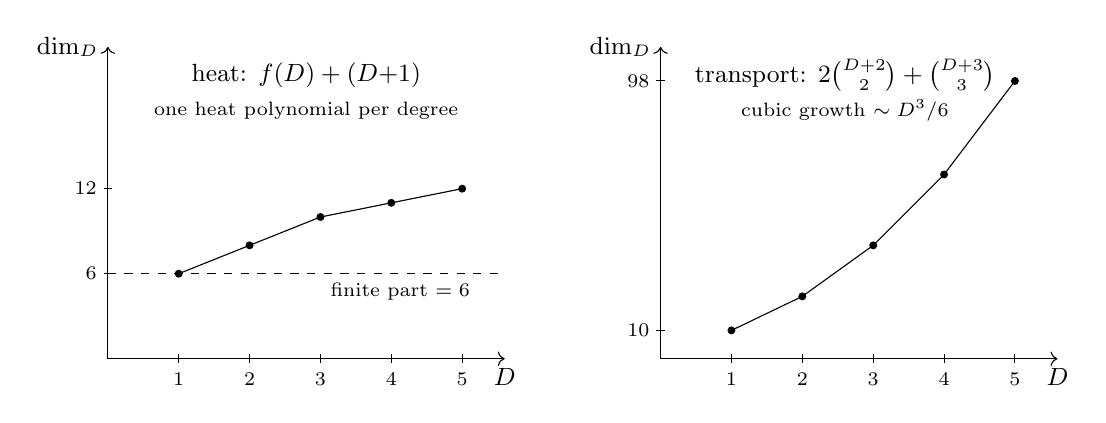
\begin{tikzpicture}[scale=0.9]
  % ---- heat staircase ----
  \begin{scope}
    \draw[->] (0.6,0) -- (6.2,0) node[below]{\small $D$};
    \draw[->] (0.6,0) -- (0.6,4.4) node[left]{\small $\dim_D$};
    \foreach \D in {1,...,5}{\draw (\D+0.6,0.06)--(\D+0.6,-0.06) node[below]{\scriptsize \D};}
    \foreach \y/\l in {1.2/6, 2.4/12}{\draw (0.54,\y)--(0.66,\y) node[left=2pt]{\scriptsize \l};}
    \draw[dashed] (0.6,1.2) -- (6.1,1.2) node[pos=0.75, below]{\scriptsize finite part $=6$};
    \foreach \D/\v in {1/6,2/8,3/10,4/11,5/12}{
      \fill (\D+0.6,{\v*0.2}) circle (1.6pt);}
    \draw (1.6,1.2)--(2.6,1.6)--(3.6,2.0)--(4.6,2.2)--(5.6,2.4);
    \node at (3.4,4.0) {\small heat: $f(D)+(D{+}1)$};
    \node at (3.4,3.5) {\scriptsize one heat polynomial per degree};
  \end{scope}
  % ---- transport staircase ----
  \begin{scope}[xshift=78mm]
    \draw[->] (0.6,0) -- (6.2,0) node[below]{\small $D$};
    \draw[->] (0.6,0) -- (0.6,4.4) node[left]{\small $\dim_D$};
    \foreach \D in {1,...,5}{\draw (\D+0.6,0.06)--(\D+0.6,-0.06) node[below]{\scriptsize \D};}
    \foreach \y/\l in {0.4/10, 3.92/98}{\draw (0.54,\y)--(0.66,\y) node[left=2pt]{\scriptsize \l};}
    \foreach \D/\v in {1/10,2/22,3/40,4/65,5/98}{
      \fill (\D+0.6,{\v*0.04}) circle (1.6pt);}
    \draw (1.6,0.4)--(2.6,0.88)--(3.6,1.6)--(4.6,2.6)--(5.6,3.92);
    \node at (3.2,4.0) {\small transport: $2\binom{D+2}{2}+\binom{D+3}{3}$};
    \node at (3.2,3.5) {\scriptsize cubic growth $\sim D^3/6$};
  \end{scope}
\end{tikzpicture}
\caption{The two measured ``infinite'' window sequences, with their closed forms
(Propositions~\ref{prop:heat} and Corollary~\ref{cor:transport}). Growth without stabilization is
the engine's \texttt{stalled} signature; these plots are that signature \emph{derived}, not merely
observed.}
\label{fig:staircase}
\end{figure}

\begin{remark}[Stress test: what the window cannot see]\label{rem:window-limit}
Stabilization is evidence, not proof. An algebra containing a generator with a non-polynomial
coefficient --- $e^{t}\partial_x$, say, or the resonant coefficients of \S\ref{sec:param} --- is
invisible at \emph{every} $D$, so $\dim_D$ can stabilize strictly below $\dim\g$. This is why the
engine's outputs carry the window tuple and why completeness claims are delegated to full
differential elimination (rif / Rosenfeld--Gr\"obner). The correct reading of every engine dim is
Lemma~\ref{lem:window}: a certified lower bound.
\end{remark}

%======================================================================
\section{The parameter: semicontinuity and the jump locus}\label{sec:param}

Fix a term-structure and let the coefficient vector $c\in\R^m$ vary (e.g.\ the family
$u_t=u+2u^3+c\,xu_x$ from the project corpus).

\begin{proposition}[Nullity jumps only up, only on thin sets]\label{prop:semi}
Let $A(c)$ be an $N\times p$ matrix whose entries are polynomials in $c$. Then there is an integer
$r^\ast$ and a proper algebraic subvariety $Z\subset\R^m$ such that
$\operatorname{rank}A(c)=r^\ast$ for all $c\notin Z$, and $\operatorname{rank}A(c)<r^\ast$ (hence
nullity \emph{strictly larger}) only for $c\in Z$.
\end{proposition}

\begin{proof}
Let $r^\ast$ be the maximal rank attained. Some $r^\ast\times r^\ast$ minor is a not-identically-zero
polynomial in $c$; let $Z$ be the common zero set of \emph{all} $r^\ast\times r^\ast$ minors. Off
$Z$ some such minor is nonzero, so the rank is $\ge r^\ast$, hence $=r^\ast$; on $Z$ every
$r^\ast$-minor vanishes, so the rank drops. $Z$ is a proper subvariety because at least one minor is
not identically zero.
\end{proof}

\begin{corollary}[Group classification, structurally]\label{cor:classification}
For a parametrized PDE family, the window dimension $\dim_D(c)$ is constant on a Zariski-open
\emph{generic branch} and increases only on the closed \emph{jump locus} $Z$. Mapping $Z$ is
exactly the classical group-classification problem (Ovsiannikov's generic/special branch splitting),
now visible as elementary linear algebra.
\end{corollary}

\begin{corollary}[The division of labor is forced]\label{cor:division}
Any predictor whose features depend only on the term-\emph{structure} (which monomials appear) is
constant in $c$, while the interesting set $Z$ has measure zero in coefficient space. Hence no
structure-based learner can detect jumps; it can at best be right generically. A learned model may
therefore \emph{order} the search (cheap, fallible); only the exact kernel computation may
\emph{assert} (Corollary~\ref{cor:valid}). This is the architecture of the project, derived rather
than decreed.
\end{corollary}

\begin{remark}[Measured instance, and the resonance mechanism]\label{rem:resonance}
In the 200-PDE corpus the audit found exactly one duplicated structure with disagreeing labels:
$u_t=u+2u^3+c\,xu_x$ with $c=-\tfrac12$ (window stable at $\dim 2$) versus $c=2$ (window growing
$2,3,4,7,13$ --- \texttt{stalled}). The mechanism: the equation is first order, so characteristics
carry exponentials $x\,e^{ct}$ and (from the Bernoulli reaction part) $e^{2t}$; polynomial symmetry
coefficients exist in quantity only when these rates combine \emph{integrally} --- $c=2$ resonates,
$c=-\tfrac12$ does not. We state this as the mechanism and flag that the full derivation of the
resonance condition is deliberately deferred; what is proved is the general shape
(Proposition~\ref{prop:semi}) and what is measured is the instance. Note also the honest subtlety:
at a resonance it is the \emph{windowed} label that jumps; deciding whether the true algebra jumps
needs escalation (higher $D$, then elimination).
\end{remark}

\begin{figure}[ht]\centering
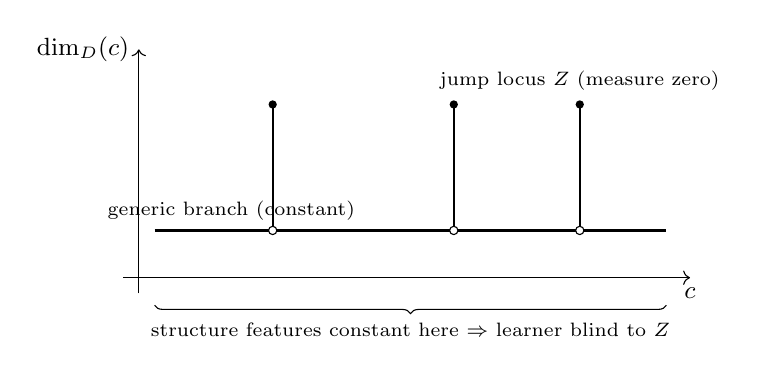
\begin{tikzpicture}[scale=1.0]
  \draw[->] (-3.4,0) -- (3.8,0) node[below]{\small $c$};
  \draw[->] (-3.2,-0.2) -- (-3.2,2.9) node[left]{\small $\dim_D(c)$};
  \draw[thick] (-3.0,0.6) -- (3.5,0.6) node[pos=0.15, above]{\scriptsize generic branch (constant)};
  \foreach \c in {-1.5, 0.8, 2.4}{
    \draw[thick] (\c,0.6) -- (\c,2.2);
    \fill (\c,2.2) circle (1.5pt);
    \draw[fill=white] (\c,0.6) circle (1.5pt);}
  \node at (2.4,2.5) {\scriptsize jump locus $Z$ (measure zero)};
  \draw[decorate,decoration={brace,mirror,amplitude=3pt}] (-3.0,-0.35) -- (3.5,-0.35)
    node[midway,below=3pt]{\scriptsize structure features constant here $\Rightarrow$ learner blind to $Z$};
\end{tikzpicture}
\caption{Semicontinuity (Proposition~\ref{prop:semi}): dimension is constant off a thin set and
jumps \emph{up} on it. Measured instance: $c=-\tfrac12$ generic, $c=2$ resonant in
$u_t=u+2u^3+c\,xu_x$. This picture is why the learned reductor is a prioritizer and never a judge.}
\label{fig:jump}
\end{figure}

%======================================================================
\section{The quotient: from kernel to reduced equation}\label{sec:quotient}

\begin{proposition}[Classical; Olver]\label{prop:reduce}
Let $X=\xi\partial_x+\tau\partial_t+\varphi\partial_u$ with $(\xi,\tau)\not\equiv(0,0)$ near a point
(\emph{transversality}). Then locally $X$ has exactly two functionally independent invariants
$z(x,t,u)$ and $W(x,t,u)$, found as first integrals of the characteristic system
$\dfrac{dx}{\xi}=\dfrac{dt}{\tau}=\dfrac{du}{\varphi}$, and the $X$-invariant solutions of a PDE
admitting $X$ are exactly the solutions of an equation in $(z,W)$ alone --- one independent variable
fewer.
\end{proposition}

The worked instance (Fisher--KPP: $X=c\,\partial_x+\partial_t$, invariants $z=x-ct$ and $U=u$,
reduced ODE $U''+cU'+U(1-U)=0$, verified symbolically and by the engine) is written out in
\texttt{intro.tex}, \S``Finding the invariants,'' and not duplicated here. Figure~\ref{fig:foliation}
draws the geometry. Two structure-theoretic facts complete the picture:

\begin{itemize}[nosep]
\item \textbf{Lie's theorem (solvability $\Rightarrow$ quadratures).} If the algebra is solvable,
  symmetries can be peeled off one at a time, each reducing the order of the reduced ODE by one ---
  when enough survive the quotient (those normalizing the used subalgebra descend), the ODE
  integrates explicitly. Fisher's reduced ODE retains the $z$-translation: that is exactly the
  license for its phase-plane analysis.
\item \textbf{Non-transversal generators reduce nothing.} A vertical generator
  ($\xi=\tau=0$) imposes the \emph{constraint} $\varphi=0$ instead of a reduction; the engine's
  refusal to reduce by such generators (returning \texttt{None}) is Proposition~\ref{prop:reduce}'s
  hypothesis enforced, not a missing feature.
\end{itemize}

\begin{figure}[ht]\centering
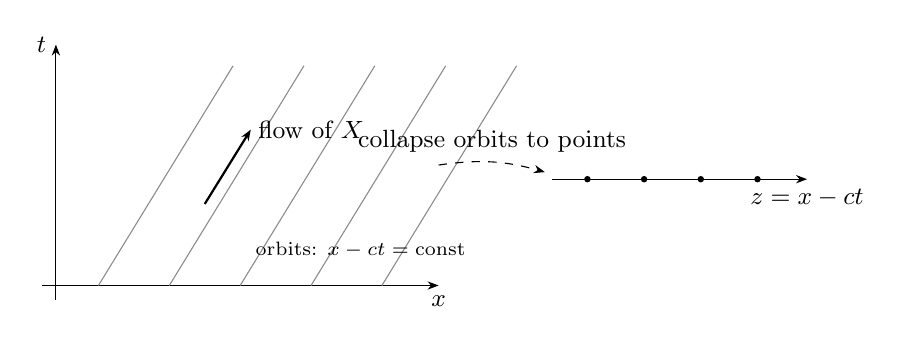
\begin{tikzpicture}[scale=0.9,>={Stealth[length=4pt]}]
  % (x,t) plane with characteristics x - ct = const
  \draw[->] (-0.2,0) -- (5.4,0) node[below]{\small $x$};
  \draw[->] (0,-0.2) -- (0,3.4) node[left]{\small $t$};
  \foreach \k in {0.6,1.6,2.6,3.6,4.6}{
    \draw[black!45] (\k,0) -- (\k+1.9,3.1);}
  \draw[->, thick] (2.1,1.15) -- (2.75,2.2) node[right=-1pt]{\small flow of $X$};
  \node at (4.3,0.5) {\scriptsize orbits: $x-ct=\mathrm{const}$};
  % quotient axis
  \draw[->] (7.0,1.5) -- (10.6,1.5) node[below]{\small $z=x-ct$};
  \foreach \z in {7.5,8.3,9.1,9.9}{\fill (\z,1.5) circle (1.3pt);}
  \draw[->, dashed] (5.4,1.7) to[bend left=12] node[above]{\small collapse orbits to points} (6.9,1.6);
\end{tikzpicture}
\caption{Reduction as geometry: the group orbits foliate the $(x,t)$ plane; the quotient is the
$z$-line; a PDE invariant along the leaves becomes an ODE on the quotient
(Proposition~\ref{prop:reduce}).}
\label{fig:foliation}
\end{figure}

%======================================================================
\section{What each result licenses the machine to do}\label{sec:license}

\begin{center}
\begin{tabular}{p{0.28\linewidth} p{0.62\linewidth}}
\textbf{Machine decision} & \textbf{Mathematical license proved or stated above}\\[2pt]
\hline\\[-8pt]
Assert ``$X$ is a symmetry'' & Corollary~\ref{cor:valid}: residual $\equiv0$ in exact arithmetic; no
learning involved, ever.\\[3pt]
Report $\dim_D$ with a window tuple & Lemma~\ref{lem:window}: monotone certified lower bound;
Props.~\ref{prop:burgers}--\ref{prop:heat}, Thm.~\ref{thm:transport}: the three G1 sequences are the
filtration doing exactly what the lemma says.\\[3pt]
Flag \texttt{stalled} instead of a number & Prop.~\ref{prop:heat}/Cor.~\ref{cor:transport}: growth
$=$ infinite part; Remark~\ref{rem:window-limit}: why stopping at a stabilized value is still only a
lower bound.\\[3pt]
Let ML \emph{order} a sweep, never filter it & Corollary~\ref{cor:division}: structure features are
blind to the jump locus by construction.\\[3pt]
Reduce only by transversal generators & Proposition~\ref{prop:reduce} and its failure mode.\\[3pt]
\hline
\end{tabular}
\end{center}

\medskip
\noindent\textbf{Verification.} Every symbolic claim in this note --- the three transport family
instances, all six classical heat generators, the six heat polynomials, and the three window
sequences against their closed forms --- is re-checked mechanically by
\texttt{symm/curriculum\_checks.py} (18/18 \textsc{pass}, exact arithmetic, no randomness). The
measured sequences themselves are pinned by the G1 regression suite
(\texttt{symm/tests/test\_textbook\_validation.py}).

\begin{thebibliography}{9}\small
\bibitem{Olver} P.~J. Olver, \emph{Applications of Lie Groups to Differential Equations}, 2nd ed.,
Springer GTM 107. (In-tree: \texttt{ref/Olver\_LieGroups\_DiffEq\_g.pdf}.)
\bibitem{Notes} \emph{Notes on Lie symmetry group methods for differential equations}. (In-tree:
\texttt{ref/Notes on Lie symmetry group methods\ldots.pdf}.)
\bibitem{Lee} J.~M. Lee, \emph{Introduction to Smooth Manifolds}. (In-tree:
\texttt{ref/lee\_smooth\_manifolds.pdf}.)
\bibitem{Hall} B.~C. Hall, \emph{Lie Groups, Lie Algebras, and Representations}. (In-tree:
\texttt{ref/Hall-LieGroupsLiealgebras2015.Springer\ldots.pdf}.)
\bibitem{Ovs} L.~V. Ovsiannikov, \emph{Group Analysis of Differential Equations}. (Unverified
bibliographic details --- cited for the classification concept; re-verify before external use.)
\end{thebibliography}

\end{document}
